%!TEX root = bambi-thesis.tex

\chapter{Pixhawk Autopilot} % (fold)
\label{appendix:pixhawk_flight_controller}
\section{Hardware} % (fold)
\label{sub:hardware}
\textit{“Pixhawk is an independent, open-hardware project aiming at providing high-end autopilot hardware to the academic, hobby and industrial communities at low costs and high availability. It provides hardware for the Linux Foundation DroneCode project. It originated from the PIXHAWK Project of the Computer Vision and Geometry Lab of ETH Zurich (Swiss Federal Institute of Technology) and Autonomous Systems Lab as well from a number of excellent individuals.”} \cite{Pixhawk}
\begin{figure}[ht]
    \centering
    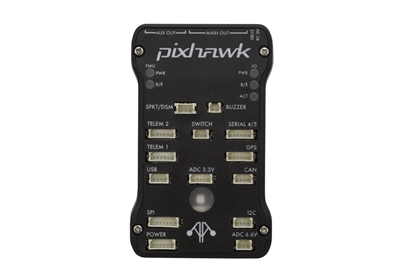
\includegraphics[width=.6\textwidth]{figures/A2/pixhawk.jpg}
    \caption{}
    \label{fig:Pixhawk Flight Controller}
\end{figure}

The Pixhawk hardware weights 38g and it is provided with a 32-bit ARM Cortex M4 core with FPU with 256 KB of RAM and a 32-bit fail-safe co-processor; it is also equipped with a compass, a barometer, an accelerometer and a gyro sensor. 
% section hardware (end)

\section{Softwere} % (fold)
\label{sub:softwere}
Modern, sophisticated flight controllers share a commonality in architecture. We can divide their functionality into three distinct layers, illustrated in \autoref{fig:FCU-architecture}.
\begin{figure}[ht]
    \centering
    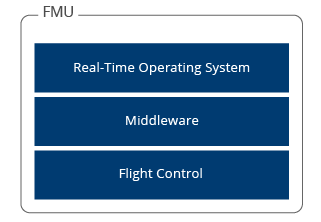
\includegraphics[width=.5\textwidth]{figures/A2/flightControllerArchitecture.png}
    \caption{The architecture of a modern flight controller}
    \label{fig:FCU-architecture}
\end{figure}
\paragraph{Layer 1: Real Time Operating System\\} % (fold)
\label{par:layer_1_real_time_operating_system}
The real time operating system is the back bone of the flight firmware, providing basic hardware abstraction and concurrency. Real time systems are critical for flight control performance and safety, as they guarantee that flight control tasks will be completed in a certain amount of time, and are essential for the safety and time-critical performance of UAVs. Luci uses a real time operating system called NuttX, which is highly expansive and configurable.
% paragraph layer_1_real_time_operating_system (end)

\paragraph{Layer 2: Middleware\\} % (fold)
\label{par:layer_2_middleware}
The middleware is a collection of tools, drivers, and libraries that relate to flight control. It contains device drivers that handle sensors and other peripherals. It also contains flight control libraries such as RC protocols, math utilities, and control filters.
% paragraph layer_2_middleware (end)

\paragraph{Layer 3: Flight Control\\} % (fold)
\label{par:layer_3_flight_control}
The flight control layer is the brains of the operation; this layer contains all of the command and control routines. Things like state estimation, flight control, system calibration, telemetry, motor control, and other flight control aspects reside in this layer.
% paragraph layer_3_flight_control (end)

\subsection{PX4 Stacks} % (fold)
\label{par:avaiable_flight_controller}

% subsection avaiable_flight_controller_ (end)
The Pixhawk platform can be flashed with two very popular flight stack: ArduPilot and PX4.
In this thesis it has been adopted the PX4 software because:
\begin{itemize}
	\item Its software-in-the-loop (SITL) simulation is much more developed and matured.
 	\item Supports a much larger number of peripherals, including more IMU sensors, lidar, range finders, status indicators, optical flow, and motion capture units. PX4 supports the most advanced sensing peripherals for drones.
 	\item Contains advanced command and control functionality, including things like terrain estimation, and indoor flight correction.
 	\item More ubiquitous and built with advanced drone applications in mind. It can be compiled for POSIX (Linux) systems, and it can also integrate with ROS to run flight applications in a hybrid system, with some running on an underlying real-time OS, and others running on Linux using ROS to communicate.
 \end{itemize} 
 The choice was mainly driven by the more developed SITL environment and framework provided by the PX4 community and for the more advanced integration with ROS rather then a matter of performance or features, where ArduPilot stack prove to be good as well.
 The diagram in \autoref{fig:PX4-architecture} provides a detailed overview of the building blocks of PX4. The top part of the diagram contains middleware blocks, while the lower section shows the components of the flight stack.
 \begin{figure}[ht]
    \centering
    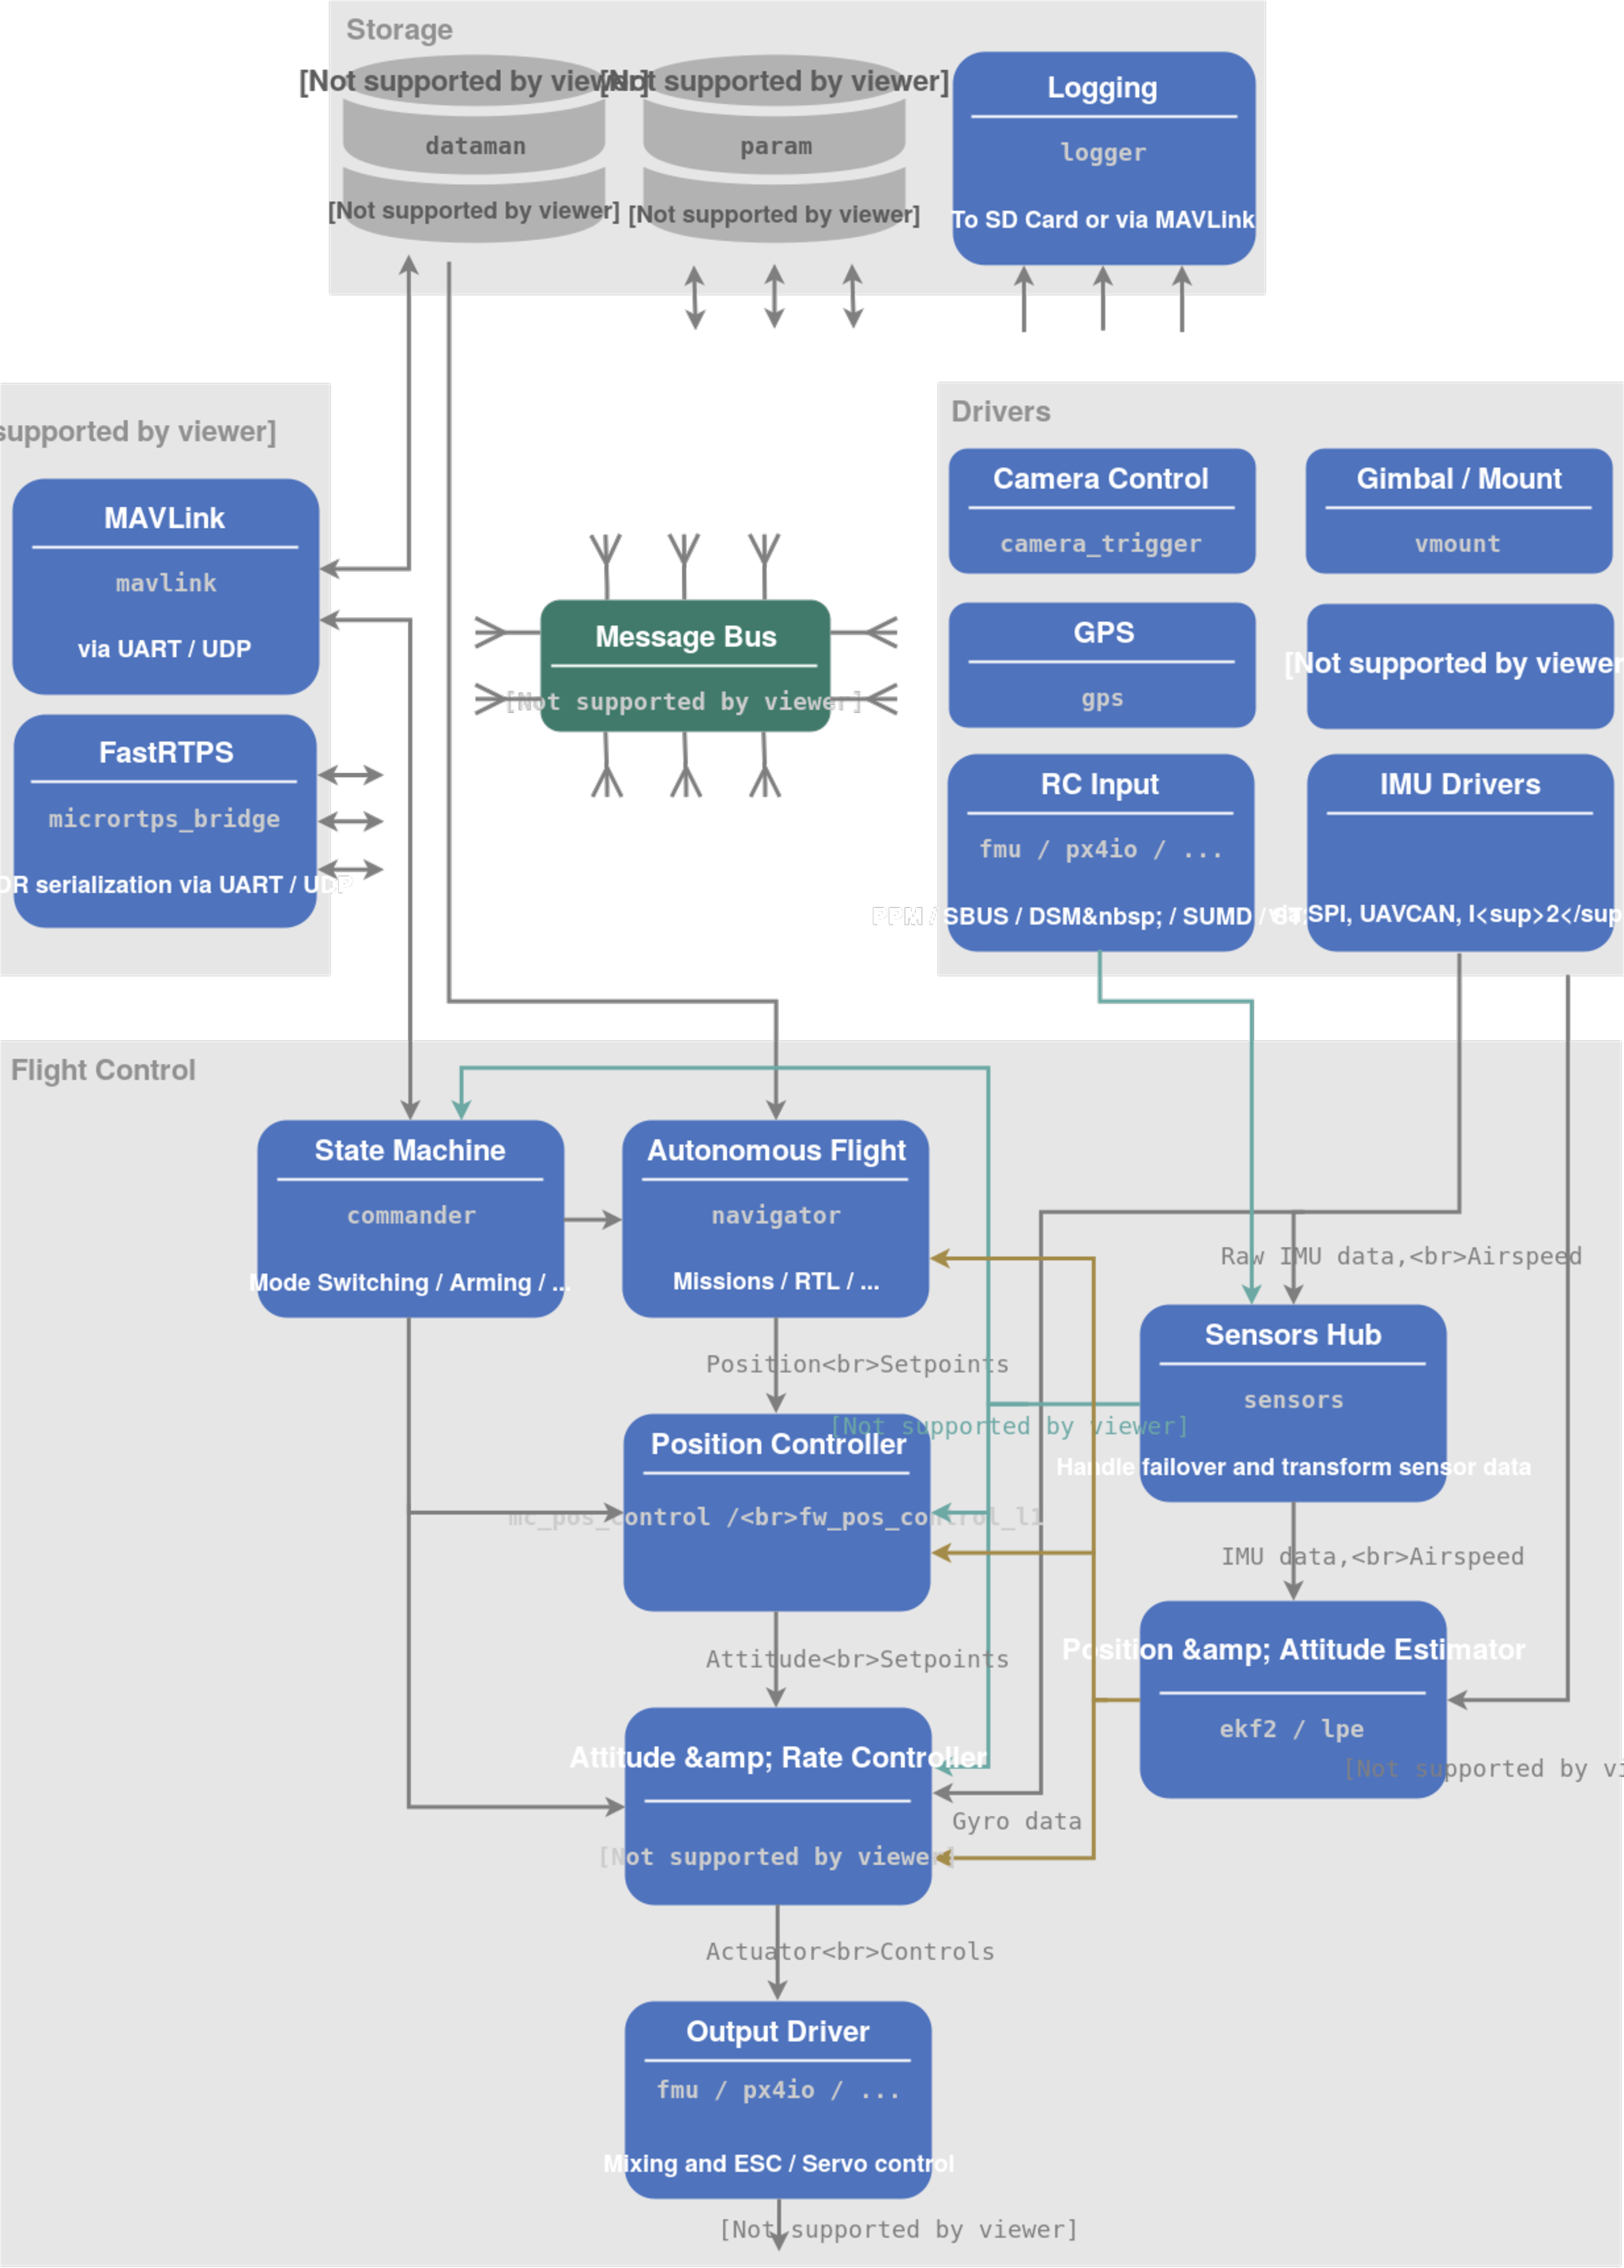
\includegraphics[width=.6\textwidth]{figures/A2/PX4_Architecture.pdf}
    \caption{PX4 Architecture}
    \label{fig:PX4-architecture}
\end{figure}
% section softwere (end)

% section pixhawk_flight_controller (end)